\cleardoublepage


\chapter{Direkte Kinematik}\label{ch:direkte-kinematik}

?? Quelle

Die direkte Kinematik ist dafür verantwortlich aus den verschiedenen Winkeln und Positionen der Gelenke die Rotation und Position des Endeffektors im Raum zu berechnen.
Dazu wird zunächst in jedem Gelenk ein Koordinatenursprung gelegt, der eine Nullstellung jedes Gelenks beschreibt.
Um alle Gelenke in einer kinematischen Kette abzubilden, kann dann beispielsweise mithilfe der homogenen Transformationsmatrix (Abschnitt~\ref{sec:homogene-transformationsmatrix}) und einem Parameter in den Freiheitsgraden des entsprechenden Gelenks eine Rechenvorschrift aufgebaut werden, um den Roboter zu beschreiben und die Position des Endeffektors schnell bestimmen zu können.


\section{DH-Konvention}\label{sec:dh-konvention}

?? Quelle

?? Unterschied UR5 und UR5e https://www.universal-robots.com/articles/ur/application-installation/dh-parameters-for-calculations-of-kinematics-and-dynamics/ ??

Die Konvention, die in der Regel verwendet wird, um Rotation und Translation eines Gliedes der kinematischen Kette darzustellen ist die sog.\ \ac{dhk} oder DH-Transformation.
\ac{dhk} beschreibt, wie die Koordinatensysteme basieren auf dem vorherigen Koordinatensystem beschrieben werden.
Um nun ausgehend von Gelenk $n-1$ das Koordinatensystem von Gelenk $n$ zu beschreiben, müssen die folgenden Regeln befolgt werden:

\begin{enumerate}
    \item Achse $z_{n}$ liegt entlang der Bewegungsachse des Gelenks $n$
    \item Achse $x_{n}$ liegt auf der kürzesten Verbindung zwischen Achsen $z_{n-1}$ und $z_{n}$.
    \item Die $y_{n}$ Achse wird rechtshändig ergänzt.
\end{enumerate}

Dabei sind die Ursprünge der Gelenkkordinatensysteme oftmals nicht im Gelenkursprung, was Komplexität für die Berechnung von Transformationen verringert.
Aus der Beziehung der zwei Koordinatensysteme können die DH-Parameter abgeleitet werden (siehe auch Abbildung~\ref{fig:dh-konvention1}):

\begin{itemize}
    \item $\theta_n$ Winkel zwischen $x_{n-1}$ und $x_n$ mit Rotationsachse $z_{n-1}$
    \item $d_n$: Kleinster Abstand zwischen $x_{n-1}$ und $x_n$
    \item $a_n$: Abstand zwischen den Achsen $z_{n-1}$ und $z_n$
    \item $\alpha_n$ Winkel zwischen $z_{n-1}$ und $z_n$ mit Rotationsachse $x_{n}$
\end{itemize}

Dies entspricht den folgenden Transformationsmatrizen (Gleichungen~\ref{eq:dh1},~\ref{eq:dh2},~\ref{eq:dh3},~\ref{eq:dh4}):

\newcommand{\ct}{\cos(\theta_n)}
\newcommand{\st}{\sin(\theta_n)}
\newcommand{\ca}{\cos(\alpha_n)}
\newcommand{\sa}{\sin(\alpha_n)}

\begin{equation}
    T_{\theta_n} =
    \begin{bmatrix}
        \ct & -\st & 0 & 0 \\
        \st & \ct  & 0 & 0 \\
        0   & 0    & 1 & 0 \\
        0   & 0    & 0 & 1 \\
    \end{bmatrix}
    \label{eq:dh1}
\end{equation}
\begin{equation}
    T_{d_n} =
    \begin{bmatrix}
        1 & 0 & 0 & 0   \\
        0 & 1 & 0 & 0   \\
        0 & 0 & 1 & d_n \\
        0 & 0 & 0 & 1   \\
    \end{bmatrix}
    \label{eq:dh2}
\end{equation}

\begin{equation}
    T_{a_n} =
    \begin{bmatrix}
        1 & 0 & 0 & a_n \\
        0 & 1 & 0 & 0   \\
        0 & 0 & 1 & 0   \\
        0 & 0 & 0 & 1   \\
    \end{bmatrix}
    \label{eq:dh3}
\end{equation}

\begin{equation}
    T_{\alpha_n} =
    \begin{bmatrix}
        1 & 0   & 0    & 0 \\
        0 & \ca & -\sa & 0 \\
        0 & \sa & \ca  & 0 \\
        0 & 0   & 0    & 1 \\
    \end{bmatrix}
    \label{eq:dh4}
\end{equation}

Um nun Koordinatensystem $n-1$ in Koordinatensystem $n$ zu überführen, kann die Transformationsmatrix $T_{n-1,n}$ verwendet werden (Gleichung~\ref{eq:dh5}).
Für den beweglichen Freiheitsgrad der Gelenke kann für die einfache Berechnung noch eine Substitution für Variable $q_n$ durchgeführt werden (Gleichung~\ref{eq:subst1} für translatorische und Gleichung~\ref{eq:subst2} für rotatorische Gelenke).

\begin{equation}
    T_{n-1,n}(q_n) \coloneqq T_{\theta_n} \cdot T_{d_n} \cdot T_{a_n} \cdot T_{\alpha_n} =
    \begin{bmatrix}
        \ct & -\st\ca & \st\sa  & a_n\ct \\
        \st & \ct\ca  & -\ct\sa & a_n\st \\
        0   & \sa     & \ca     & d_n    \\
        0   & 0       & 0       & 1      \\
    \end{bmatrix}
    \label{eq:dh5}
\end{equation}

?? Modifizierte dh-parameter, andere Matrix (siehe andersen~\cite{rasmusandersenKinematicsUR52018})

\begin{figure}[h]
    \centering
    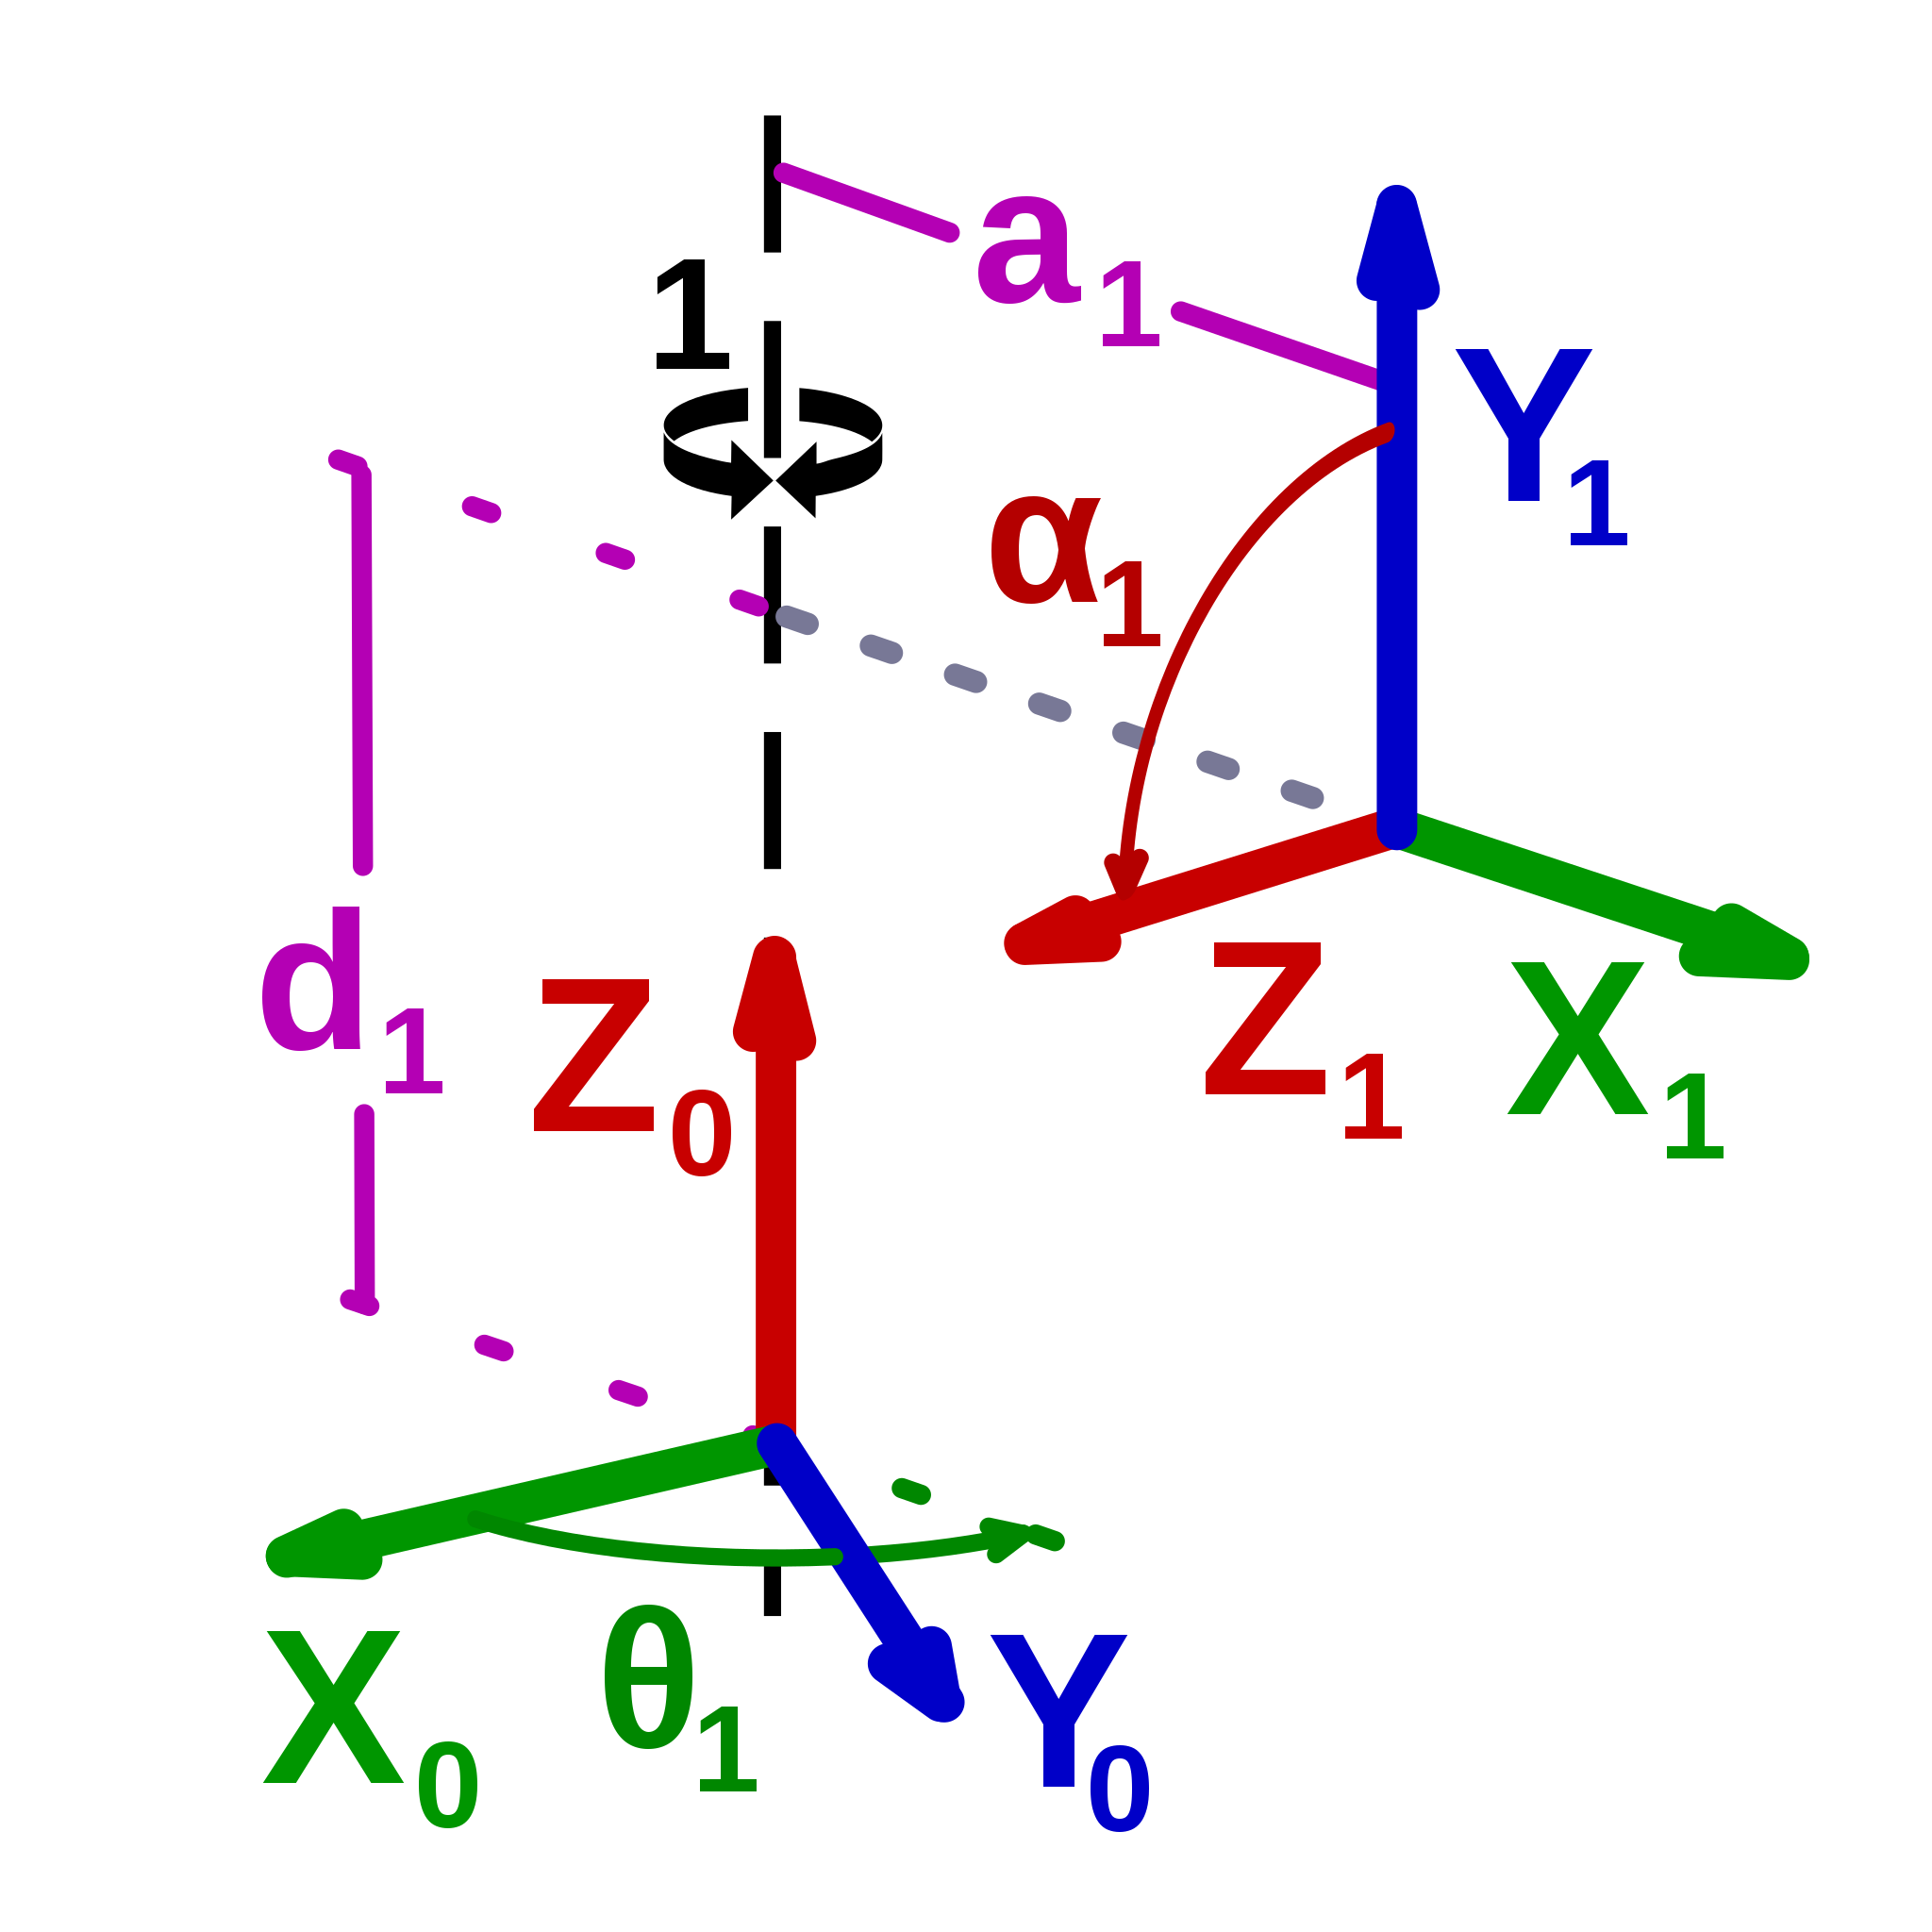
\includegraphics[width = .5\textwidth]{Bilder/Denavit-Hartenberg-Transformation.svg}
    \caption{\ac{dhk} zwischen zwei Gelenken~\cite{jahobrCoordinateSystemsDenavitHartenberg2007}}\label{fig:dh-konvention1}
\end{figure}


\begin{equation}
    d_n \coloneqq d_{n_0} + q_n    \label{eq:subst1}
\end{equation}
\begin{equation}
    \theta_n \coloneqq \theta_{n_0} + q_n    \label{eq:subst2}
\end{equation}


\section{Unified Robot Description Format}\label{sec:urdf}

?? Quelle
\ac{urdf} ist ein Standard entwickelt für \ac{ros}, um sowohl die geometrischen als auch physische und visuelle Eigenschaften eines Roboters zu beschreiben.
Für die Beschreibung ist eine auf XML basierende Datei nötig, die mit Tags geschachtelt den Roboter mithilfe von sog. \enquote{links} und \enquote{joints} beschreibt.

Links beschreiben die physischen Verbindungen zwischen zwei Gelenken.
Dabei wird unterschieden zwischen visuellen Eigenschaften (\enquote{visual}), Kollisionseigenschaften (\enquote{collision}) und Trägheitseigenschaften (\enquote{inertial}).
Jede dieser Kategorien kann so die Geometrie des Links aus verschiedenen Perspektiven unterschiedlich beschreiben

Joints bezeichnen Gelenke, also die Verbindungen zweier Links und beschreiben die mögliche relative Bewegung zwischen diesen.
Dabei sind nicht nur translatorische (\enquote{prismatic}) und rotatorische Gelenke (\enquote{revolute}) beschreibbar, sondern auch feste (\enquote{fixed}), schwebende (\enquote{floating}) und planare Verbindungen (\enquote{planar}).
Für die Beschreibung eines Joints wird der vorhergehende Link als \enquote{parent} und der nächste Link als \enquote{child} bezeichnet.
Zudem müssen im Feld \enquote{origin} Translation und Rotation des Ursprungs im Koordinatensystem des Parent Links, sowie im Feld \enquote{axis} je nach Gelenk die Rotationsachse, Translationsachse oder Normale der Bewegungsoberfläche angegeben werden.
Desweiteren ist es möglich, Schnittstellen für die Bewegung der Motoren zu definieren und Bewegungslimits für die Gelenke anzugeben, um die Ansteuerung des Roboters und die Bewegungsplanung zu vereinfachen.


\section{Beschreibung des UR5e}\label{sec:ur5-in-dh}
?? Quelle https://www.universal-robots.com/articles/ur/application-installation/dh-parameters-for-calculations-of-kinematics-and-dynamics/

Der in dieser Arbeit betrachtete Roboter ist der UR5e von Universal Robots.
Dieser ist ein vergleichsweise günstiger Roboter mit verringerter Zahl an Singularitäten (siehe Abschnitt~\ref{sec:singularitaten}), sechs Gelenken und einer offenen kinematischen Kette.
Offiziell wird der Roboter mit den DH-Parametern aus Tabelle~\ref{tab:ur5-dh1} und dynamischen Eigenschaften der Links aus Tabelle~\ref{tab:ur5-dh2} beschrieben.
Abbildung~\ref{fig:ur5-axis} kann zudem die Dimensionierung des Roboters und die Anordnung der Achsen in Nullstellung entnommen werden.

\begin{figure}[h]
    \centering
    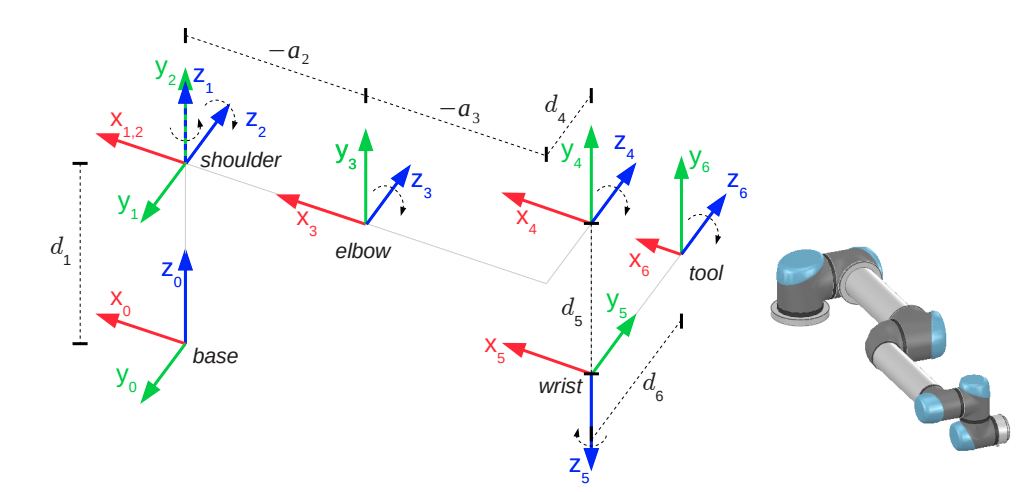
\includegraphics[width = .9\textwidth]{Bilder/ur5-axis}
    \caption{Achsen des UR5-Roboters mit Angabe der DH-Parameter (links) und Visualisierung der Nullposition (rechts)~\cite{rasmusandersenKinematicsUR52018}}\label{fig:ur5-axis}
\end{figure}

\begin{table}
    \centering
    \begin{tabular}{lrrrllrl}
        \toprule
        \textbf{Joint} & $\boldsymbol{\theta}$ \textbf{[rad]} & $\boldsymbol{a}$ \textbf{[m]} & $\boldsymbol{d}$ \textbf{[m]} & $\boldsymbol{\alpha}$ \textbf{[rad]}  \\
        \midrule
        Joint 1        & 0                                    & 0                             & 0.1625                        & \pi/2                                \\
        Joint 2        & 0                                    & -0.425                        & 0                             & 0                                    \\
        Joint 3        & 0                                    & -0.3922                       & 0                             & 0                                    \\
        Joint 4        & 0                                    & 0                             & 0.1333                        & \pi/2                                \\
        Joint 5        & 0                                    & 0                             & 0.0997                        & -\pi/2                               \\
        Joint 6        & 0                                    & 0                             & 0.0996                        & 0                                    \\
        \bottomrule
    \end{tabular}
    \caption{DH-Parameter des UR5e Roboters von Universal Robots~\cite{UniversalRobotsDH}}
    \label{tab:ur5-dh1}
\end{table}
\begin{table}
    \centering
    \begin{tabular}{lrrrllrl}
        \toprule
        \textbf{Link} & \textbf{Masse [kg]} & \textbf{Schwerpunkt [m]} \\
        \midrule
        Link 1        & 3.761               & [0, -0.02561, 0.00193]   \\
        Link 2        & 8.058               & [0.2125, 0, 0.11336]     \\
        Link 3        & 2.846               & [0.15, 0.0, 0.0265]      \\
        Link 4        & 1.37                & [0, -0.0018, 0.01634]    \\
        Link 5        & 1.3                 & [0, 0.0018,0.01634]      \\
        Link 6        & 0.365               & [0, 0, -0.001159]        \\
        \bottomrule
    \end{tabular}
    \caption{Beschreibung der dynamischen Eigenschaften des UR5e Roboters von Universal Robots~\cite{UniversalRobotsDH}}
    \label{tab:ur5-dh2}
\end{table}